\acresetall
\chapter{Schizophrenia}
\label{ch:intro:scz}
\section*{Overview}
\Scz/ is a chronic, debilitating disease affecting approximately 1\% of the worldwide population \citep{NIMHb}.
In the United States, it is estimated that 20\% of all \scz/ patients are homeless and \scz/ is associated with an approximately 20 year reduced life expectancy.
\todo[color=green]{Find homeless and life expectancy reference}
A 2011 World Economic Forum report \citep{Bloom2011} estimated that the global burden of mental illness -- of which \scz/ is a major contributor -- would be more than 16~trillion~US\$ over the next 20 years, or approximately 1-2\% of the 2010 global GDP per year.
Compared to all other non-communicable diseases, mental illness accounts for the most lost output, more than cardiovascular disease and cancer (\autoref{fig:intro:scz:output_loss}).
For \scz/ in particular, the cost of \scz/ in the United States was estimated to reach \$155~billion in 2013, 24\% going to direct cost of treatment, and 75\% coming from indirect costs including caregiving for patients and unemployment \citep{Cloutier2016}. 
\begin{figure}
	\centering
	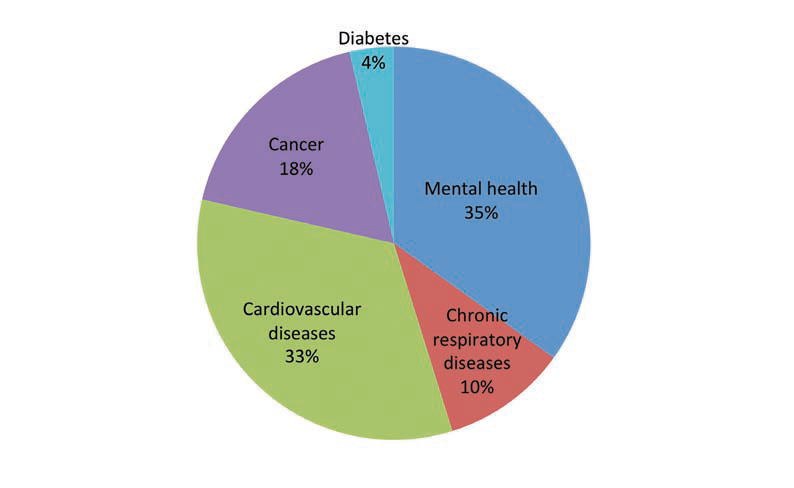
\includegraphics[width=0.7\textwidth]{intro/Bloom2011_output_loss_by_NCD}
	\caption[Breakdown of non-communicable disease cost by disease type]{Breakdown of non-communicable disease cost by disease type. Reproduced from \citet{Bloom2011}.}
	\label{fig:intro:scz:output_loss}
\end{figure}

\Scz/ is a syndrome defined by its symptoms, the most prominent of which is psychosis.
Symptoms are generally classified into three main categories: positive, negative, and cognitive \citep{Kay1982, NIMHa}.
Positive symptoms are behaviors not normally seen in healthy individuals and include hallucinations, delusions, suspiciousness, hostility, thought disorders, and movement disorders.
Negative symptoms reflect missing or disrupted normal thought processes, including: blunted affect, social withdrawal, avolition, anhedonia, and difficulty in abstract thinking.
Cognitive symptoms include attentional deficits, poor executive functioning, both working and long-term memory impairment, specifically in the domains of episodic semantic memory deficits.
While the positive symptoms, in particular hallucinations and delusions, might be the most prominent symptoms of \scz/, cognitive symptoms are present in up to 75\% of \scz/ patients and the severity of cognitive symptoms is strongly linked to functional outcomes \citep{O'Carroll2000, Green1996, Keefe2007}.
This is particularly troubling since treatment options for the negative and cognitive symptoms of \scz/ are extremely limited.

Since the underlying causes of \scz/ are not known, treatment for patients with \scz/ is limited to treating symptoms as they present.
Treatment for \scz/ patients primarily includes a combination of antipsychotic medication and psychosocial therapy \citep{NIMHa}.
Patients' responses to antipsychotics varies widely, some experiencing complete remission of psychoses and others showing no alleviation of symptoms.
Overall, following a first episode-psychosis, long-term antipsychotic treatment are effective in 30-40\% of patients in preventing future psychoses \citep{Boyer2007, Insel2010}, leaving over half of all patients still experiencing psychotic episodes.
More importantly, antipsychotic medication only aim to treat the positive symptoms of \scz/, such as hallucinations and delusions.
There are limited treatment options for the debilitating cognitive deficits -- including deficits in attention, executive function, and both working and episodic memory -- which have proven to be the greatest barrier to rehabilitation \citep{Lieberman2005, Harrison2001, O'Carroll2000, Hyman2003}.

Like most mental disorders, the underlying etiology of \scz/ is most likely complex and heterogeneous, making the discovery of a single `monotherapy' unlikely \citep{Hyman2003}.
For these reasons, there is growing appreciation that we need to better understand and treat sets of symptoms separately, particularly developing new drug interventions for the negative and cognitive symptoms of \scz/.
Indeed, it seems likely that what today we call \scz/ is in fact a collection of related disorders, some potentially common to other mental health disorders as well \citep{Insel2010}.
This view of \scz/ implies that by focusing on particular dysfunctions -- such as episodic memory impairment -- we can hope to find general therapeutic targets for diseases currently classified separately, and at the same time, by looking for convergence on to common endophenotypes we can identify treatment targets shared by patients with heterogeneous underlying etiology.

In the following sections I will expand upon some of the symptoms, brain abnormalities, and causative factors observed in \scz/ patients, with a specific focus on aspects of the disease most relevant to my main research project (see \autoref{ch:df}).
I will discuss details of the memory deficits present in \scz/ patients [\ref{sec:intro:scz:memory}], with a particular focus on spatial and episodic memory impairments.
% I will present what we do know about underlying genetic and environmental causes of \scz/ [\ref{sec:intro:scz:genes_and_environment}], including details of 22q11.2 deletion syndrome and a mouse model of this deletion, \df/.
I will present what we know about specific brain regions affected in \scz/ patients, specifically focusing on the \ac{HPC} [\ref{sec:intro:scz:brain}].
Finally, I will lay out several proposed causes of \scz/ symptoms including genetic risk factors, alterations in neumodulatory signaling, and an imbalance in excitation and inhibition [\ref{sec:intro:scz:etiology}].

\section{Memory deficits}\label{sec:intro:scz:memory}
Disruption in working and declarative memory are among the primary cognitive deficits observed in \scz/ patients.
The memory deficits present in \scz/ are specific in that patients seem to have relatively spared implicit or procedural memory, while many patients present with striking deficits in declarative memory (see \autoref{sec:intro:memory:memory}), including both episodic memory -- conscious recollection of events -- and semantic memory -- knowledge of people, place, objects, and facts \citep{O'Carroll2000, Aleman1999, Gold2010}.
In addition to being specific, the observed memory deficits are also pervasive, in that they can not be accounted for by age, education, medication, disease duration or severity \citep{Ranganath2008} and are present in the majority of \scz/ patients.
\todo[color=green]{cite prevalence of memory deficits in SCZ patients}
As mentioned more generally about cognitive symptoms of \scz/, the severity of memory impairments in particular is one of the strongest predictors of longterm functional outcome among \scz/ patients \citep{Green1996}, as failures in declarative memories provide the greatest barrier to steady employment.

The pattern of memory deficits observed in \scz/ patients is consistent with disruptions in both the executive control and memory strategies associated with the \ac{PFC} as well as with the longterm memory storage function of the \ac{HPC}.
Disorders that specifically arise from \ac{PFC} lesions or dysfunction show a similar impairment in encoding and retrieval as seen in \scz/ patients \citep{Ranganath2008}.
Patients do not make use of the same semantic memory strategies as healthy individuals, though these impairments can at least in part be ameliorated by training or through restructuring of task stimuli (e.g. blocked instead of unblocked word lists) \citep{Gold1992, Stone1998}.

\subsection{Spatial memory}\label{sec:intro:scz:spatial}
As described in more detail above (see \nameref{sec:intro:memory:spatial-episodic}), memory for specific locations is one particular type of episodic memory that has proven to be a tractable means for studying memory.
While less recognized as a core symptom of \scz/, spatial memory deficits are well documented in \scz/ patients \citep{Boyer2007, Hanlon2006, Wilkins2013, Weniger2008}, but the underlying circuit level dysfunctions have rarely been investigated \citep{Hayashi2015, Suh2013}.
A lack of general awareness of spatial memory deficits in \scz/ patients is most likely attributable to the different approaches taken by clinical psychologists and basic research scientists.
Deficits in verbal memory are among the most prominent cognitive deficits observed in \scz/ patients \citep{O'Carroll2000}.
The broad category of verbal memory reflects the nature of psychological tests used to assess memory deficits, they involve verbal discourse with the clinician.
In practice verbal memory tests generally test either short-term working memory -- with tests such as the Digit Span test which probes the number of items that one can remember and immediately recall -- or longterm declarative memory.
Longterm declarative memory tests includes remembering lists of potentially semantically grouped lists or aspects of narrative stories.
This longterm declarative memory component of verbal memory tests (referred to as \textsc{secondary verbal memory}) is particularly impaired in \scz/ patients \citep{Green1996}.

In addition, the deficits observed in spatial memory seem to be specific to allocentric navigation, as compared to egocentric navigation.
For example, a study by \citeauthor{Wilkins2013} used a 4-on-8 virtual maze to distinguish between allocentric (referred to as `spatial') and egocentric (`response') navigation strategies \citep{Wilkins2013}.
The 4-on-8 virtual maze places participants in a virtual 8-arm radial maze with distal landmarks visible around the maze.
In the first phase of the task 4 arms are blocked and the participants travel to the end of the 4 open arms to receive rewards.
In the second phase all 8 arms are opened and the participants must learn to travel down the 4 newly-available arms to retrieve rewards.
Finally, in the probe trials, all 8 arms are open, with rewards in the original 4 open arms, but now the walls of the arms are raised to occlude the distal landmarks.
During these probe trials, participants who learned an egocentric strategy (e.g. visit the 1\super{st}, 3\super{rd}, 5\super{th}, \& 6\super{th} arms clockwise around the maze.) would still perform well, but those who learned an alocentric strategy (e.g. rewards are near the mountain, forest, lake, and sun.) would perform poorly.
The authors found that \scz/ patients who used an allocentric navigation strategy performed significantly worse than healthy controls, but patients who used an egocentric navigation strategy performed similar to health individuals.
This differential effect was also seen in learning to navigate a virtual park versus a virtual maze \citep{Weniger2008} and in a virtual Morris water maze comparing hidden- and visible-platform trials \citep{Hanlon2006}.
In agreement with the well-characterized hippocampal deficits in \scz/ patients (see \autoref{sec:intro:scz:hpc}), allocentric navigation is \acs{HPC}-dependent (see \autoref{sec:intro:memory:spatial}), while egocentric navigation primarily relies on the caudate nucleus \citep{Hartley2003}.

\section{\Scz/ in the brain}\label{sec:intro:scz:brain}
% \subsection{Anatomy}

% HPC
% PFC
% STRIATUM

Brain structural changes have been reliably identified in \scz/ patients following a first episode of psychosis, and more recently, in high-risk individuals during the prodrome, prior to a clinical diagnosis.
In particular, reductions in gray matter volume and a corresponding increase in lateral ventral volume have been consistently demonstrated \citep{Fusar-Poli2013, Shepherd2012}.
As we become aware of susceptibility genes, environmental triggers, and other prodromal markers of \scz/, the identification of an at-risk pool has allowed for the tracking of brain changes prior to the onset of psychosis.
Tracking of clinically high-risk individuals has identified \scz/-related structural changes in the hippocampal formation, the cerebellum, the superior and medial temporal lobe, the insular cortex and the \ac{PFC} \citep{Cannon2015, Millan2016}.
Additionally, among the clinically high-risk population, continued progression towards \scz/ can be predicted by monitoring gray-matter loss \citep{Tognin2014}, aiding in pre-symptomatic identification with the hope of early intervention treatments (see \nameref{sec:intro:scz:neurodevelopment}).

\subsection{Hippocampus}\label{sec:intro:scz:hpc}
Of particular relevance to my primary thesis project, consistent behavioral, anatomical, and physiological studies of \scz/ patients have all pointed towards the HPC as an integral region in disease pathology \citep{Boyer2007, Bogerts1985, Jakob1986}.
Meta-analysis of quantitative \ac{fMRI} studies found overall significant effect sizes of 0.37 and 0.39 for the left and right \ac{HPC} respectively, corresponding to an approximately 4\% reduction in bilateral hippocampal volume \citep{Nelson1998}.
There was no effect of duration of illness, which also adds further support for the neurodevelopmental etiology of \scz/ (see \autoref{sec:intro:scz:neurodevelopment}), as that implies that either the \ac{HPC} suddenly reduces in volume by 4\% on the day of first-episode psychosis or the hippocampal volume reduction is already present prior to clinical disease onset. 

Of these subcortical projections the medial septum projections are of particular interest, since the cholinergic projection has been linked to learning and memory \citep{Parent2004} and the GABAergic projection is known to target PV+ interneurons \citep{Freund1988} which are altered in \scz/ (see \nameref{sec:intro:scz:glutamate}) and it has also been linked to aberrant behavior in an NMDAR antagonist model of schizophrenia \citep{Ma2012}.
Despite these well-characterized features of hippocampal organization, it remains unknown how the function of these circuit motifs are altered in \scz/ during hippocampal-dependent behaviors.

\subsubsection{CA1}
There is growing evidence that hippocampal area CA1 is the first subregion affected in \scz/, and potentially the source of hippocampal deficits.
Work by \citeauthor{Schobel2009} used high-resolution (sub-millimeter pixel size) \ac{fMRI} of baseline activity to compare \scz/ patients to healthy controls.
The authors particularly looked at regions previously associated with \scz/ (the hippocampal formation, frontal cortex, basal ganglia, and amygdala) and found a preferential increase in \ac{CBV} in \scz/ patients in hippocampal area CA1 and orbitofrontal cortex, and a decrease in dorsolateral \ac{PFC} \citep{Schobel2009}.
In addition, the authors followed a prodromal population over two years and found that baseline \ac{CBV} abnormalities specifically in hippocampal area CA1 predicted progression to psychosis.
Finally, symptom severity was also shown to correlate with \ac{CBV} levels in area CA1.
Follow-up work showed that hippocampal hypermetabolism spread from CA1 to other regions, prodromal CA1 hypermetabolism predicted post-psychosis hippocampal atrophy, and linked deficient glutamate levels (see \autoref{sec:intro:scz:glutamate}) to the observed effects \citep{Schobel2013}.
Similarly, a recent study found that progressive hippocampal area CA1 volume loss correlated with disease progression and it spread from CA1 to other hippocampal subfields \citep{Ho2017}.
Finally, in my primary research project (\autoref{ch:df}) I investigated the role of aberrant CA1 activity in spatial memory disruptions in a mouse model of \scz/, which further adds evidence for a central role of hippocampal area CA1 in \scz/.

\subsubsection{CA2}
\todo[inline, color=yellow]{Discuss CA2 in SCZ?}

\subsection{Prefrontal cortex}
\todo[inline, color=yellow]{Discuss PFC in SCZ?}

\section{\Scz/ etiology}\label{sec:intro:scz:etiology}
While the underlying cause of schizophrenia has remained elusive, collective evidence has pointed to several possible mechanistic pathways.
Narrowing down the disease etiology has been confounded by a high concordance with other psychiatric diseases \citep{Kessler2005}.
Unlike Alzheimer’s disease or Parkinson’s disease where cell-death of specific cell types has been causally linked to disease progression, \scz/ and many other psychiatric disorders exhibit no drastic cell loss or increased gliosis, and affected brain regions can span both cortical and subcortical regions, suggesting network or circuit dysfunctions \citep{Uhlhaas2012, Lewis2002}.
A clear genetic-risk component has been recognized for quite some time, which is perhaps most evident by an exponentially increasing risk for developing \scz/ with relatedness to a \scz/ patient \citep{Rodriguez-Murillo2012}, but other risk factors are now becoming better understood as well, including shared family environment, male gender, advanced paternal age, perinatal events, and substance abuse \citep{Lichtenstein2009}.

\subsection{Genetics}
Current estimates suggest that \scz/ has up to 80\% heritability arising from a large network of genetic abnormalities that predispose for \scz/ \citep{Ripke2011}, though most \scz/ patients do not in fact have a family history of \scz/ \citep{Rodriguez-Murillo2012}.
This suggests that either \scz/ risk is conferred by many genes that individually have minimal effect, so go unnoticed unless combined with other risk factors, or highly-penetrant individual mutations that are quickly selected against but arise \emph{de novo} leading to \scz/.
% The search for genetic risk factors has focused on several approaches, primarily genome-wide association studies (GWAS), case-studies of familial-\scz/ linked to specific highly-penetrant mutations, and newer assays for copy-number variants (CNVs) among \scz/ patients.
Linkage-based analysis has identified over 1000 proposed genes associated with \scz/, but many of these findings have failed to be replicated and their validity is questionable \citep[\url{http://www.szgene.org}, ][]{Allen2008}.
More recent analysis has focused on un-biased genome-wide investigations
Advances in sequencing technologies now allows for the sequencing of large portions of the genome of \scz/ patients, which has aided the search for copy-number variants (CNVs), single-nucleotide variations (SNVs), smaller insertions/deletions \citep{Rodriguez-Murillo2012}.
\todo[color=red]{expand on scz genetics}

\subsubsection{Gene pathway convergence}
\todo[inline, color=yellow]{write genetic pathway convergence section}

\subsubsection{22q11.2 deletion syndrome}
Perhaps the best-established and well-studied CNV linked to \scz/ is a deletion present in human chromosome 22 (22q11.2) \citep{Karayiorgou1995, Chow2006, Karayiorgou2010}.
Individuals with 22q11.2 deletions exhibit a spectrum of cognitive deficits as children, and $~$30\% of them develop \scz/ in adolescence or early adulthood, accounting for up to 2\% of all \scz/ cases \citep{Karayiorgou2010}.
\todo[color=green]{Expand on 22q11.2}

\subsubsection{\df/}
Advances in understanding the genetic component of \scz/ predisposition have led to the development of etiologically-validated mouse models of \scz/ which will allow for the direct analysis of \emph{in vivo} neuronal network activity and identification of circuit dysfunctions present in the disease.
In order to dissect altered hippocampal circuitry in \scz/ I will be using the etiologically validated mouse model of the 22q11.2 microdeletion (\df/), generated by deleting the syntenic region in the mouse chromosome which contains most of the same 28 genes deleted in humans \citep{Stark2008}.
\begin{figure}
	\centering
	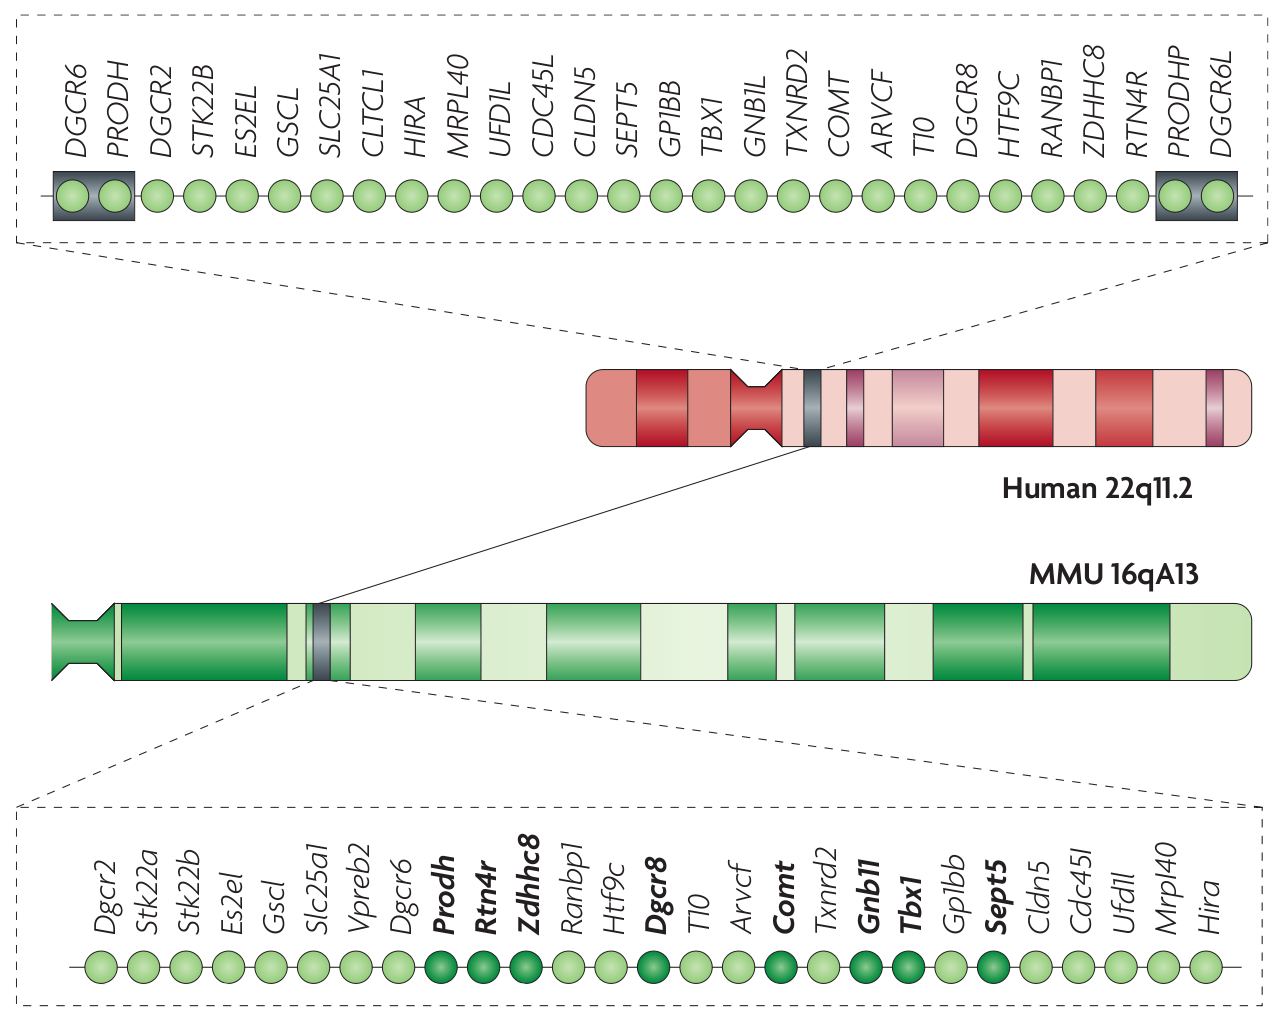
\includegraphics[width=0.8\textwidth]{intro/22q11ds_genes}
	\caption[Genetic deletion in 22q11.2DS and \df/]{Genes involved in the human 22q11.2 deletion and syntenic region in the mouse genome. Modified from \citet{Karayiorgou2010}}
	\label{fig:intro:scz:22q11_genes}
\end{figure}

Behavioral tests on the \df/ mouse model have shown increased non-specific anxiety in open field and light-dark transition tasks, impaired sensorimotor gating by measuring startle response during prepulse inhibition (PPI), impaired spatial working memory in a delayed non-matching to place T-maze task, impaired working memory, and decreased freezing in a contextual fear conditioning paradigm, which could reflect either impaired contextual memory or the inability to associate the unconditioned stimuli with the context in which it was presented \citep{Drew2011b, Stark2008, Sigurdsson2010}.
Additionally, a study of immediate early gene expression using c-Fos staining following exposure to a novel environment found significantly fewer CA3 pyramidal cells active and a trend in the same direction for CA1 pyramidal cells as well, which is suggestive of deficits in spatial memory \citep{Drew2011b}.
Finally, recent work in the \df/ mouse has identified a hippocampal area CA2-specific reduction in PV+ interneurons, a corresponding decrease in inhibitory activity onto CA2 pyramidal cells, and a deficit in CA2-dependent social memory \citep{Piskorowski2016}.

\emph{In vivo} neurophysiology experiments have additionally identified several deficits in this mouse model.
In a paper by \citeauthor{Sigurdsson2010}, the authors found that synchrony between the \ac{HPC} and \ac{PFC} was disrupted in the \df/ mouse model during a working memory task that generally relies on increased synchrony between those two brain regions and in which the \df/ mice showed a learning deficit \citep{Sigurdsson2010}.
In addition, they found that baseline synchrony predicted later task performance, suggesting a basal disruption in functional connectivity.
More recently, \citeauthor{Hamm2017} recorded neuronal activity in primary visual cortex of \df/ mice and found several indications for altered local coordination and synchrony among the neuronal population, leading to the hypothesis that disrupted local attractors lead to aberrant activity in \scz/ \citep{Hamm2017}.

Taken together, the \df/ mouse model of the human \scz/-linked 22q11.2 microdeletion effectively recapitulates cognitive deficits seen in \scz/ patients, including increased anxiety, impaired executive control, and deficits in spatial and episodic memory.
Modeling these cognitive deficits in a mouse model allows us to directly investigate underlying cellular and circuit dysfunctions, a topic I will discuss in detail in \autoref{ch:df}.

% \subsection{Schizophrenia as a neurodevelopmental disorder}\label{sec:intro:scz:neurodevelopment}

% The typical age for a first psychotic episode is 18-25 years, though there is 
% \begin{figure}
% 	\centering
% 	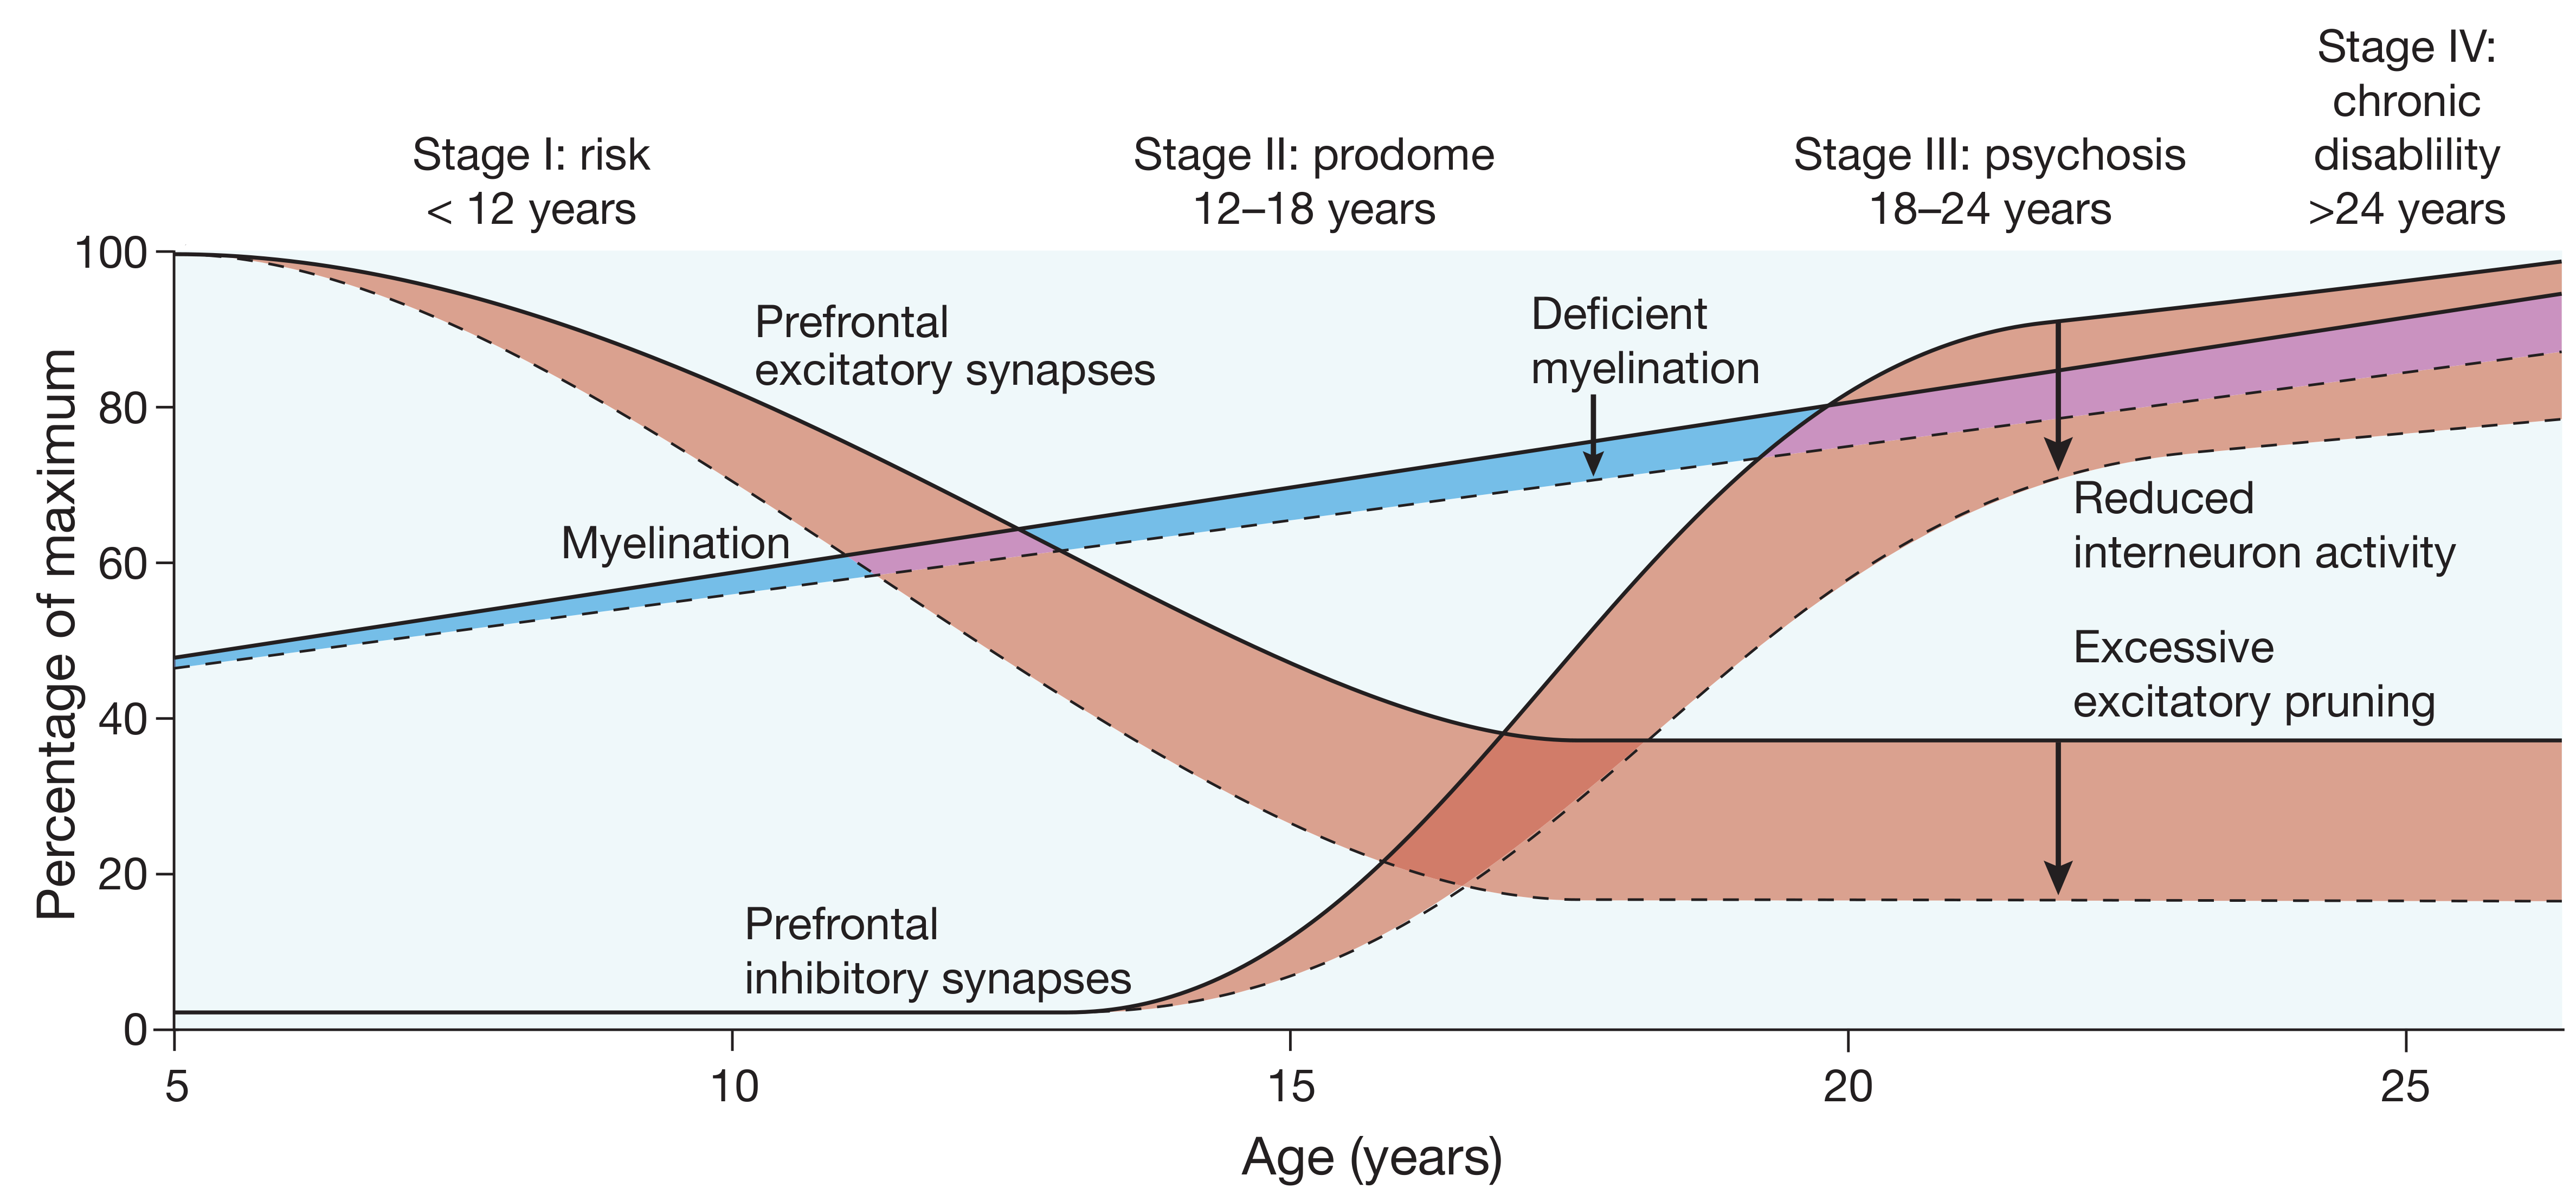
\includegraphics[width=0.9\textwidth]{intro/Neurodevelopmental_model}
% 	\caption[Neurodevelopmental model of \scz/]{Neurodevelopmental model of \scz/. Reproduced from \citet{Insel2010}}
% 	\label{fig:intro:scz:neurodevelopmental}
% \end{figure}

\subsection{Dopamine}
The earliest mechanistic hypotheses for the disease progression of \scz/ involves disruption in normal dopamine signaling \citep{Matthysse1973}.
This hypothesis revolves around the positive symptoms of \scz/, specifically the hallucinations and delusions which can be both induced and prevented through modification of dopamine levels in the brain.
In particular, compounds that generally increase the level of dopamine (e.g. amphetamine, LSD) lead to hallucinations similar to those experienced by \scz/ patients \citep{Angrist1994, Lieberman1987}.
Conversely, for over 60 years the primary treatment for \scz/ has been antipsychotic medications \citep{Delay1952}, which were first shown to increase the metabolism of dopamine \citep{Carlsson1963} and are now known to function primarily as D2 dopamine receptor antagonists \citep{}.
The general effectiveness of classical antipsychotics (e.g. haloperidol) and the newer atypical antipsychotics (e.g. clozapine) in treating the positive symptoms of \scz/, suggested a central role for dopamine in the more general neuropatholysiology of \scz/, but this insight has failed to expand beyond the direct treatment of psychotic episodes.
Indeed, while D2 dopamine receptor antagonists work well for many patients in managing psychotic episodes, these treatments have done very little in improving functional outcomes, as the more debilitating negative and cognitive symptoms remain untreated \citep{Insel2010}.

The role of dopamine in \scz/ is now realized to be more nuanced than a simple consequence of a brain-wide hyperdopaminergic state.
While D2 dopamine receptor antagonist antipsychotic treatments do help manage psychotic episodes in many \scz/ patients, in some these treatments show no effect.
Additionally, post-mortem measurements of dopamine levels in \scz/ patients, as well as \emph{in vivo} measurements of dopamine activity, have not been entirely consistent across studies, and more importantly, across patients \citep{}.
This inconsistency is most likely reflective of variability in underly disease etiology, and points to a lack of a singular disease pathology, but rather a collection of underlying brain dysfunctions that funnel towards shared pathways and a commonly identified set of expressed symptoms.

Using radiolabeled L-dopa, presynaptic dopamine levels have been consistently shown to be elevated in the striatum of \scz/ patients \citep[for review, see][]{Howes2007}
At the same time, also in the striatum, D2/3 dopamine receptors (the primary receptor subtypes in this brain region) are modestly (10-20\%) elevated, independent of treatment with antipsychotic drugs \citep[for review, see][]{Howes2009}.
In contrast to the striatum, D1 dopamine receptors predominantly mediate dopamine activity, and while the effect is not as consistent, receptor levels show an association with severity of cognitive and negative symptoms in \scz/ \citep{Goldman-Rakic2004}.

\subsubsection{Dopamine in the striatum}
One brain region in particular, the striatum, has been particularly identified as a potential target region for altered dopamine signaling. Studies in human patients have found evidence for increased dopamine uptake in the striatum, and post-mortem studies have found elevated dopamine and dopamine metabolite levels in the striatum \citep{Simpson2010}.
In addition, post-mortem studies have reported increased levels of dopamine D2 receptors in un-medicated human patients compared to unaffected controls, suggesting a possible source of dopamine mis-regulation and a potential molecular target for manipulation and translation in to a valid animal model \citep{}.

Previous studies by \citeauthor{Kellendonk2006} have characterized a striatal dopamine hyper-activity mouse model that over-expresses the dopamine D2 receptor (D2R-OE) specifically in the striatum \citep{Kellendonk2006}.
They showed that increased D2R activity in the striatum leads to deficits in \ac{PFC}-dependent working-memory tasks and an increased dopamine-induced excitability in \ac{PFC} cells.
The mesolimbic pathway is a potential mechanism of action, where striatal medium spiny neurons (MSNs) have altered excitability due to over-expression of D2Rs which then project to the ventral tegmental area (VTA) dopaminergic neurons, which in turn project to the \ac{PFC}, which feeds back on to striatal MSNs.
Recent work has shown that both the tonic and burst firing rates of VTA neurons are altered, though neurons in the substantia nigra (SN) are unaffected, despite both being dopaminergic centers that receive strong projections from the striatum \citep{Krabbe2015}.


% D2r presynaptic striatum

% hypodopamine frontal?

% dopamine spcific to psychoses

% many underlying causes that converge on dopamine (complex genetic interactions and environmental hits)

% subcortical hyperdopaminergia, prefrontal hypodopaminergia

\subsection{Glutamate/GABA}\label{sec:intro:scz:glutamate}
It has been proposed that an imbalance in levels of excitatory and inhibitory activity during development underlies \scz/ \citep{Insel2010, Coyle2006, Yizhar2011}.
Similar to how the effectiveness of D2 dopamine-receptor targetting antipsychotics gave rise to the "dopamine hypothesis" of \scz/, one of the main pieces of evidence in support of a "glutamamte hypothesis" of \scz/ etiology is the effect of NMDAR-receptor modulators in \scz/ patients.
NMDA receptor (NMDAR) antagonists, such as phencyclidine and ketamine, induce psychoses in healthy subjects reminiscent of hallucintations observed in \scz/ patients \citep{Javitt1991, Krystal1994} and have also been shown to present similar spatial memory deficits as \scz/ patients along with corresponding aberrant activity in the hippocampus \citep{Morgan2014}.
\Scz/ patients are particularly sensitive to the effect of these drugs, as they worsen psychotic events.
In addition, NMDAR-antagonists induce \scz/-like symptoms in mice \citep{Inta2010}.
Finally, despite poor blood-brain barrier penetrance, NMDAR-agonists significantly improve negative symptoms in \scz/ patients, and specifically drugs targeting the NMDAR glycine binding site show potential to alleviate symptoms \citep{Tsai1998, Coyle2012}.

\todo[inline, color=red]{Tonegawa nmdar ko mouse model}
% Coyle2012 Postmortem studies and NMDAR as part of a circuit

Postmortem analysis has found mixed, but generally not robust, changes in NMDAR levels in \scz/ patients relative to healthy controls.
Additionally, postmortem studies have found decreased levels of pre-synaptic GABAergic machinery, including GAT, GAD67, and parvalbumin (PV), in both the \ac{PFC} and HPC \citep{Coyle2006, Zhang2002, Konradi2011}.
In particular, \scz/ patient have shown decreased levels of parvalbumin leading to hypofunction of PV+ interneurons in the \ac{PFC} as well as decreased numbers of PV+ interneurons in the HPC \citep{Zhang2002, Lewis2005} and parvalbumin interneurons are required for normal spatial working memory functions \citep{Korotkova2010, Murray2011}.
However, there is currently limited data available on how the activity of hippocampal GABAergic interneurons is altered in \scz/.
